% !TEX root = twe2.tex

\section{Diskussion}
\label{sec:Disukussion}
\textcite[33-36]{weggler2050leguminosen} hat Möglichkeiten zur Steigerung der \ac{NEL}-Erträge im Grünland Mithilfe von Rot- und Weißlklee untersucht.
Obwohl die \ac{NEL}-Erträge gesteigert werden konnten, sanken teilweise die \ac{NEL}-Gehalte (siehe \cref{subsec:NEL}).
\textcite{fritz2018wirtschaftliche} haben gezeigt, dass die Ernteverluste bei modernen Ernteverfahren bei etwa 20\% liegen.

%, allerdings ist zu beachten, dass aktuelle Verfahren der Futterkonxerierung zu hohen Verlusten führen, siehe \cref{subsec:Lit:Ernte}.
%Mit zukünftigen Ernte- und Konservierungsverfahren werden Landwirte hoffentlich Möglichkeiten haben die Verluste zu reduzieren.

\subsection{Literaturkritik}
\label{sub:kritik}

\begin{figure}
	\centering
	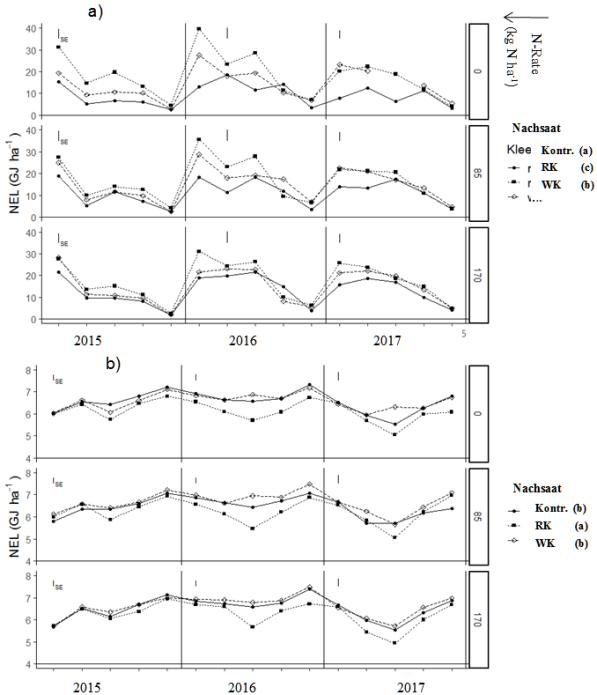
\includegraphics[width=0.8\textwidth]{images/wegglerAbb1}
	\caption[(a) \acs{NEL}-Ertrag und (b) \acs{NEL}-Konzentration in Abhängigkeit von der N-Düngung und Leguminosen Nachsaat über 3 Jahre]{(a) \ac{NEL}-Ertrag und (b) \ac{NEL}-Konzentration in Abhängigkeit von der N-Düngung und Leguminosen Nachsaat über 3 Jahre \parencite[35]{weggler2050leguminosen}}
	\label{fig:wegglerAbb1}
\end{figure}



Die Arbeit von \textcite{weggler2050leguminosen} richtet sich eindeutig an ein wissenschaftliches Fachpublikum.
Die Veröffentlichung erfolgte im Zuge der 63. Jahrestagung der \ac{AGGF} auf welcher sich Wissenschaftler über die Zukunft des Grünlandes ausgetauscht haben.
Das Thema \ac{NEL}-Ertragssteigerung über die Nachsaat von Klee in Grünlandbeständen wurde bisher wissenschaftlich kaum betrachtet (siehe \cref{subsec:NEL}).
In dem Artikel \parencite[33-36]{weggler2050leguminosen}\todo{Seitenangabe notwendig wenn die komplette Arbeit referenziert wird?} sind einige kleinere handwerkliche Fehler enthalten.

Aufgrund der begrenzten Länge in dem Tagungsband erfolgt die Darstellung der Daten, wie in wissenschaftlichen Veröffentlichungen üblich, sehr kompakt und auf das Wichtigste reduziert.
Für Wissenschaftler, welche das Fachgebiet kennen, sind solche Einschränkungen kein Problem.
Allerdings ist es für Landwirte nur schwer die Ergebnisse korrekt zu interpretieren.

In \textcite[35]{weggler2050leguminosen} ist die Legende sowie Achsbeschriftung, siehe \cref{fig:wegglerAbb1}, nicht korrekt umgesetzt.
%\todo{Numerierung ok? Verwendung Abk ok?, Breite ok? Müssen Abb. linksbündig sein?}
So wird zum Beispiel der \ac{NEL}-Gehalt mit GJ\,ha\textsuperscript{-1} beschrfitet, statt MJ\,kg\textsuperscript{-1} \ac{TM}.

Des weiteren wird die Abkürzung \ac{NEL} in der Einleitung nicht als \acl{NEL} eingeführt sondern als \textit{nutzbare Energie Laktation}.\todo{kursiv okay zum markieren von Fehlern?}
Im Kapitel Material und Methoden wird \ac{NEL} als \textit{Netto Energie Lactation} bezeichnet.
In Abbildungsunterschriften wird wiederholt \textit{nutzbare Energie Laktation} verwendet.
Normalerweise wird im landwirtschaftlichen Kontext die Abkürzung \acs{NEL} für \acl{NEL} verwendet.
Des weiteren ist \ac{NEL} eine wichtige Kenngröße in der Grundfuttermittelproduktion der Milchkuhhaltung und somit der Grünlandwirtschaft.
Daher liegt es nahe einen Fehler in der Bezeichnung zu vermuten.

%Die Darstellung der \cref{fig:wegglerAbb1} ist nicht ideal.
%Die verschiedenen Messpunkte beziehen sich auf die einzelnen Aufwüchse, diese per Linie miteinander zu verbinden hilft zwar beim erkennen welcher Punkt zu welcher Datenreihe gehört, aber die Messdaten haben nicht die Aufgabe.
%Es gitb aber keine Datenpunkte welche zwischen den einzelnen Aufwüchsen liegt, welche man eventuell interpolieren könnte.
%Wen die x-Achse die N-Düngung angeben würde und die verschiedenen Schnitte in mehrere Diagramme aufgeteil worden wären, wobei bei jedem Schnitt jeweils der Durchschnitt der 3 Jahre genommen wird, wäre die Darstellung leichter verständlich.





\subsection{Sinnhaftigkeit einer Leguminosennachsaat}
\label{sub:leguminosen}
Wie in \cref{subsec:Protein} gezeigt, können Leguminosen den \ac{XP}-Ertrag vom Grünland erhöhen.
Der Versuch von \textcite{weggler2050leguminosen} wurde allerdings nur bis zu einer Düngung von 170\,kg\,N\,ha\textsuperscript{-1}a\textsuperscript{-1} gesteigert.
Daher ist es schwierig, einen Vergleich zwischen einer, in Norddeutschland üblichen,\todo{Zitat einfügen} N-Düngung von über 200\,kg\,N\,ha\textsuperscript{-1} sowie einer minimierten N-Düngung mit Leguminosen zu ziehen.
Eine Nachsaat mit Rotklee hatte häufig einen negativen Einfluss auf den \ac{XP}-Gehalt des Aufwuchs, während eine Weißlkleenachsaat tendenziell eine leichte Steigerung des \ac{XP}-Gehaltes zur Folge hatte.
Wie in \cref{subsub:alternative} gezeigt wird, ist der \ac{NEL}- und \ac{XP}-Gehalt eine sehr wichtige Größe in der Milchkuhhaltung. 
Generell sind deutliche Steigerungen des \ac{NEL}-Ertrages möglich, insbesondere bei (sehr) geringer N-Düngung, wobei insbesondere der Rotklee dies über die Steigerung der \ac{TM}-Erträge (siehe \cref{subsec:TM}) erreicht.

Das der Rotklee zu einer signifikanten Verringerung der \ac{NEL}-Konzentration des Aufwuchses geführt hat, ist für Milchkuhbetriebe nachteilig.
Aufgrund der geringeren \ac{NEL}-Konzentration ist davon auszugehen, dass die Milchleistung der Milchkühe nachlässt.
%Daher scheint eine Strategie mit einer Rot- und Weißklee Mischung als Nachsaat für die meisten Betriebe eine Option zu sein.
Bei Betrieben, welche eine etwas geringere Viehbesatzdichte haben, kann eine Weißkleenachsaat sinnvoller sein, da in diesem Fall geringere \ac{TM}-Erträge nicht so stark ins Gewicht fallen, aber die leicht gestiegen \ac{XP}- und \ac{NEL}-Gehalte Vorteile bringen können.
In weiteren Forschungen können die betriebswirtschaftlichen Einflüsse auf die Betriebe ausgearbeitet werden um den Beratern von milchkuhhaltenden Betrieben eine wissenschaftlich fundierte Empfehlung geben zu können.
Des weiteren könnte untersucht werden, ob unterschiedliche Rotkleesorten unterschiedliche \ac{NEL}-Gehalte aufweisen oder ob z.B. andere Schnittzeitpunkte den \ac{NEL}-Gehalt steigern können.

\subsubsection{Nährstoffkreislauf}
\label{subsub:nährstoffkreislauf}

In der Milchkuhhaltung besteht, wie in \cref{subsec:Stickstoff} gezeigt, ein Nährstoffkreislauf.
Dabei ist eine sehr große N-Quelle das Kraftfutter und das Milcheiweiß eine entsprechende N-Senke.
%Über den Verkauf von Milch verlassen Nährstoffe, insbesondere N in Form des Milcheiweißes, den Betrieb.
%Falls der Betrieb den Wirtschaftsdünger abgibt, bzw. abgeben muss, verlassen darüber weitere Nährstoffe den Betrieb, unter anderem N.
%Nährstoffeinträge sind insbesondere über den Zukauf von Kraftfutter sowie, in eher geringen Mengen, der Einsatz von mineralischen Düngemitteln.
%Der Einsatz von Kraftfuttern ist für eine Milchkuh zur Steigerung der Milchleistung sehr sinnvoll.
%Eine Redufzierung des Kraftuffters ist, in den meisten Fällen, unwirtschaftlich.

Bei einer Reduzierung der N-Düngung auf den betriebseigenen Grünlandflächen ist, in den meisten Fällen, nicht mehr genügend (Acker-)Fläche vorhanden, um die eigenen Wirtschaftsdünger innerhalb des Betriebes zu verwerten.
Aufgrund der hohen Transportkosten ist eine Verwertung im nahem Umkreis anzustreben.
Insbesondere in Regionen mit einer hohen Tierdichte entsteht somit ein Überschuss an Wirtschaftsdüngern welcher auf Kosten der Tierhalter exportiert werden müsste.
Dies ist für die dort angesiedelten Betriebe eine große wirtschaftliche Herausforderung.
Nicht nur aufgrund der Transportkosten, welche in der Regel der abgebende Betrieb tragen muss, sondern auch, weil auch andere wichtige Nährstoffe abgegeben werden und somit wieder zugekauft werden müssten.

Das von \textcite[33]{weggler2050leguminosen} angebrachte Argument, dass der Kraftfuttereinkauf gesellschaftlich kritisch gesehen wird und gesenkt werden sollte, muss umgesetzt werden, damit die Leguminosennachsaat sinnvoll wird.
Nur wenn weniger Stickstoff über das Kraftfutter in den Nährstoffkreislauf eingetragen wird, ist ein N-Eintrag über Leguminosen im Sinne der N-Bilanz sinnvoll.

\subsubsection{Leguminosen als alternative zu Kraftfutter}
\label{subsub:alternative}
Bei einem Einsatz von Leguminosen in der Grundfuttergewinnung ist, wie in \cref{subsec:NEL} gezeigt, eine Steigerung der \ac{NEL}-Erträge möglich.
Aufgrund der relativ hohen Fixkosten für Stallgebäude und ähnliche Einrichtungen ist in der Milchkuhhaltung eine hohe Milchleistung sehr wichtig für die Wirtschaftlichkeit der Milchkuhhaltung.
Eine Reduzierung der Kraftfuttergabe ist, zu mindestens für die meisten Betriebe mit intensiver Milchkuhwirtschaft, aufgrund der deutlich geringeren Milchleistung der Milchkühe, nicht wirtschaftlich.
Für die Milchleistung ist der \ac{NEL}-Gehalt der Ration ein sehr wichtiger Parameter welcher über das Kraftfutter deutlich erhöht wird.
Wenn zudem das Grundfutter auch einen geringeren \ac{NEL}- und \ac{XP}-Gehalt hat, sinkt die Milchleistung noch stärker. \todo{Zitat}
%Über das Kraftfutter wird kein Raufutter substituiert, daher ist der Einsatz von Kraftuffter unabhängig von der Qualität des Raufutters zu bewerten.

Falls die Kraftfutterkosten so weit steigen, dass dieses nur noch eingesetzt werden, um eine möglichst tiergerechte Ration zu erstellen, dann würde eine große N-Quelle für die Milchkuhhaltung zu einer kleinen werden.
Ein ähnlicher Effekt würde entstehen, wenn aufgrund gesetzlicher Regelungen die Kraftfutterfütterung von Wiederkäuern eingeschränkt werden würde.
%, kann es sein, dass der Einsatz nicht mehr wirtschaftlich sinnvoll ist.
%Eine andere  wäre, dass die \ac{EU} z.B. den Kraftfuttereinsatz in der Wiederkäuerfütterung einschränken könnte.
Da insbesondere Soja aus Südamerika, momentan eine der wichtigsten \ac{XP}-Quellen \todo{zitat} der Milchkuhhaltung, gesellschaftlich in der Kritik steht, kann es passieren, dass die \ac{EU} entsprechende Schritte unternimmt.

Für den Fall dass der Eintrag von N über das Kraftfutter in den Nährstoffkreislauf deutlich reduziert wird, ändern sich die Voraussetzungen.
Da der Verlust über den Verkauf von Milch bestehen bleibt, müssen neue N-Quellen erschlossen werden.
Eine Möglichkeit ist der Einsatz von mineralischen N-Düngemitteln, eine andere Möglichkeit wäre der Einsatz von Leguminosen.
In diesem Fall, je nach Entwicklung der Preise und basierend auf den Ergebnissen von \textcite[33-36]{weggler2050leguminosen}, könnte eine Leguminosennachsaat wirtschaftlich sinnvoll sein.


\subsection{Effizienz der Konservierung}
\label{sub:konservierung}
\ac{NEL}-Verluste während der Ernte, Konservierung oder Lagerung verschlechtern die Wirtschaftlichkeit enorm.
Nachdem der Landwirt aufwändig hochwertiges Futter erzeugt hat, verliert dieser etwa 20\% des \ac{NEL}-Ertrags von der Mahd bis zum Futtertisch.
Eine Optimierung der Prozesse für eine bessere Konservierung könnte sehr positive Auswirkungen auf die Wirtschaftlichkeit entsprechender Betriebszweige haben.
%Die Reduzierung dieser Verluste wird immer wichtiger, da vermutlich größere Anteile der \ac{NEL} über das Grundfutter abgedeckt werden muss.
Eine Verbesserung der Ernteverfahren bzw. Konservierungsmethoden ist daher anzustreben.
Bestimmte Ernteverfahren stellen Ansprüche an den Grünlandaufwuchs, so muss eine Silage so gut verdichtet sein, dass keine Luft vorhanden ist bzw. eindringen kann.
Bei einer Heutrocknung ist eine gute Durchlässigkeit der Luft im Heustock anzustreben, sodass z.B. der Einsatz von Rotklee den Trocknungserfolg positiv beeinflussen kann.
Dies führt zu unterschiedlichen Ansprüchen an den Aufwuchs und somit auch an die Gräsermischung.
Somit ist eine ganzheitliche Betrachtung der Grundfutterproduktion anzustreben, auch wenn der Aufwand sehr hoch ist.
%Es bleibt somit zu hoffen dass die Forschung neue wirtschaftliche Verfahren entwickelt welche eine wirtschaftliche Nutzung des kompletten \ac{NEL}-Ertrags von landwirtschaftlichen Flächen erlaubt.

\section{Fazit}
\label{sec:fazit}
Mithilfe von Rotklee kann der \ac{NEL}-Ertrag des Grünlandes deutlich gesteigert werden.
Allerdings geht dies zu Lasten des \ac{NEL}-Gehaltes, sodass unter den aktuellen Rahmenbedingungen der Einsatz einer Rotkleenachsaat für die meisten Betriebe keinen wirtschaftlichen Vorteil bringen dürfte.
Für Betriebe, welche vor der Wahl stehen ihre \ac{TM}-Erträge steigern zu müssen oder weniger Tiere zu halten, könnte eine Rotkleenachsaat sinnvoll sein.
Alle Alternativen sollten allerdings betriebsindividuel wirtschaftlich duchgerechnet werden um eine gute Grundlage für eine Entscheidung zu haben.

Neben der Steigerung der \ac{NEL}-Erträge wäre eine effizientere Konservierung dieser wünschenswert.
Allerdings hat die Gräsermischung einen sehr großen Einfluss auf die Qualität der Futterkonservierung, sodass eine Betrachtung verschiedener Verfahren in Verbindung mit unterschiedlichen Grünlandbeständen sinnvoll erscheint.
Aufgrund der Komplexität des Themas, ist ein Vergleich unterschiedlicher Strategien sehr schwierig.
